
\section{Experimento BRDF Oren-Nayar} \label{section-experiment-oren-nayar}

Este experimento é baseado no trabalho de Oren e Nayar \cite{oren1994generalization}, no qual propuseram uma generalização do modelo de refletância de Lambert, desenvolvendo uma abordagem matemática para modelar com maior precisão a difusão de luz em superfícies rugosas. As equações que descrevem esse experimento se encontram na \autoref{fig-oren-nayar-eqlang-latex}. O código-fonte em \texttt{EquationLang}, usado como entrada para o compilador, está dividido em duas partes: a primeira no \autoref{cod-oren-nayar-eqlang-pt-1} e a segunda no \autoref{cod-oren-nayar-eqlang-pt-2}. A renderização dos objetos 3D utilizando essa BRDF está na \autoref{fig-oren-nayar-eqlang}, e os \textit{plots} correspondentes estão na \autoref{fig-oren-nayar-plots}. A saída em GLSL está dividida em três partes: a parte 1 no \autoref{cod-oren-nayar-glsl-pt-1}, a parte 2 no \autoref{cod-oren-nayar-glsl-pt-2}, e a parte 3 no \autoref{cod-oren-nayar-glsl-pt-3}.


%%%%%%%%%%%%%%%%%%%%%%%%%%%%%%%%%%%%%%%%%%%%%%%%%
\subsection{Representação em documento \LaTeX{}}
%%%%%%%%%%%%%%%%%%%%%%%%%%%%%%%%%%%%%%%%%%%%%%%%%
\begin{figure}[H]
    \caption{\label{fig-oren-nayar-eqlang-latex} 
    \small Equações da BRDF do experimento Oren-Nayar em documento \LaTeX{}.}
    \begin{center}
        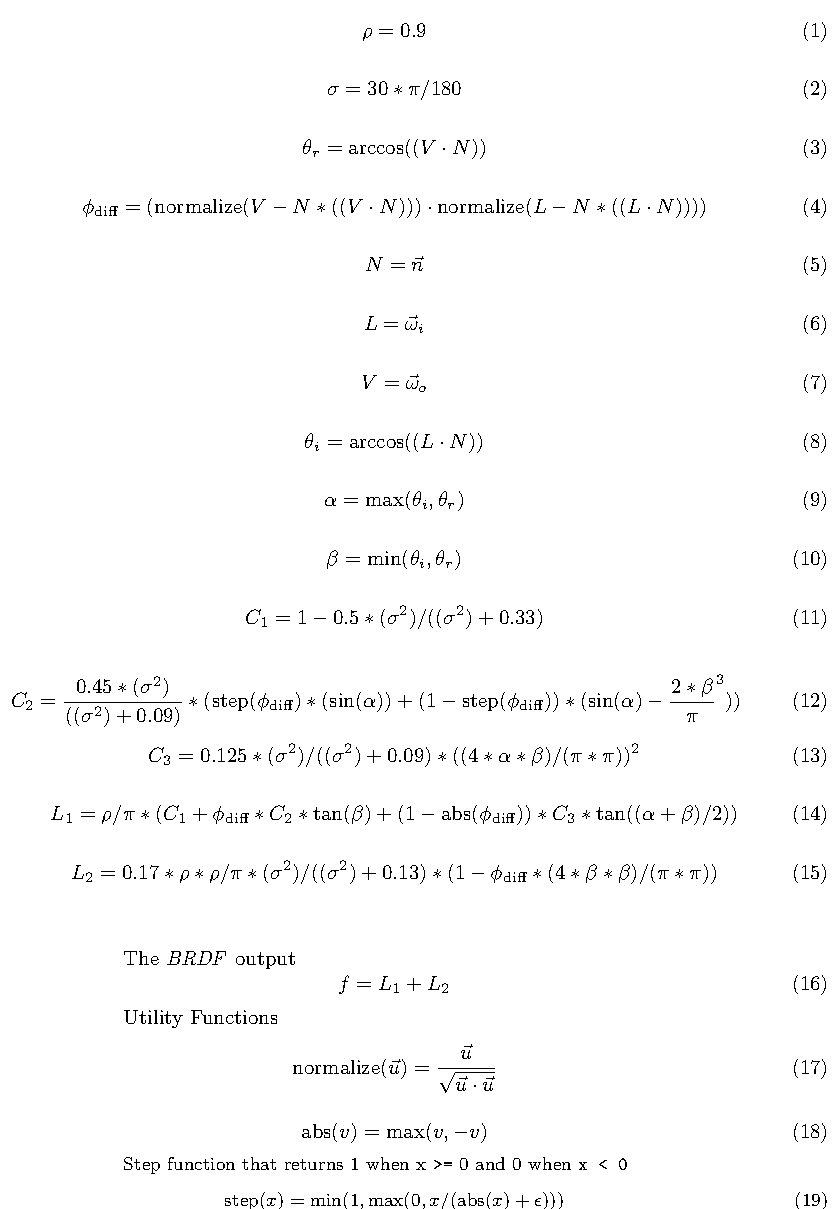
\includegraphics[scale=0.82]{./Imagens/brdfs/oren-nayar.pdf}
    \end{center}
\end{figure}

%%%%%%%%%%%%%%%%%%%%%%%%%%%%%%%%%%%%%%%%%%%%%%%%%
\subsection{Código Fonte em \texttt{EquationLang}}
%%%%%%%%%%%%%%%%%%%%%%%%%%%%%%%%%%%%%%%%%%%%%%%%%
\begin{codigo}[H]
    \caption{\small Código fonte da BRDF do experimento Oren-Nayar (parte 1 de 2).}
    \label{cod-oren-nayar-eqlang-pt-1}
\begin{lstlisting}[language=tex, frame=none, inputencoding=utf8]
\begin{equation}
    \rho = 0.9
\end{equation}
\begin{equation}
    \sigma = 30*\pi/180
\end{equation}
\begin{equation}
    \theta_r = \arccos((V \cdot N))
\end{equation}
\begin{equation}
    \phi_{\text{diff}} = ( \text{normalize}(V-N*((V \cdot N))) \cdot \text{normalize}(L - N*((L \cdot N))) )
\end{equation}
\begin{equation}
    N = \vec n
\end{equation}

\begin{equation}
    L = \vec \omega_i
\end{equation}

\begin{equation}
    V = \vec \omega_o
\end{equation}

\begin{equation}
    \theta_i = \arccos ((L \cdot N))
\end{equation}

\begin{equation}
    \alpha = \max (\theta_i, \theta_r)
\end{equation}

\begin{equation}
    \beta = \min (\theta_i, \theta_r)
\end{equation}

\begin{equation}
    C_1 = 1 - 0.5 * (\sigma^2) / ((\sigma^2) + 0.33)
\end{equation}

\end{lstlisting}
\end{codigo}

\begin{codigo}[H]
    \caption{\small Código fonte da BRDF do experimento Oren-Nayar (parte 2 de 2).}
    \label{cod-oren-nayar-eqlang-pt-2}
\begin{lstlisting}[language=tex, frame=none, inputencoding=utf8]
\begin{equation}
    C_2 = \frac{0.45 * (\sigma^2)}{ ((\sigma^2) + 0.09)}
        * (
            \text{step}(\phi_{\text{diff}})       * (\sin(\alpha))
            + (1 - \text{step}(\phi_{\text{diff}}))  * (\sin(\alpha) - \frac{2*\beta}{\pi}^3)
        )
\end{equation}
\begin{equation}
    C_3 = 0.125 * (\sigma^2) / ((\sigma^2)+0.09) * ((4*\alpha*\beta)/(\pi*\pi))^2
\end{equation}

\begin{equation}
    L_1 = \rho/\pi * (C_1 + \phi_{\text{diff}} * C_2 * \tan(\beta) + (1 - \text{abs}(\phi_{\text{diff}})) * C_3 * \tan((\alpha+\beta)/2))
\end{equation}

\begin{equation}
    L_2 = 0.17 * \rho*\rho / \pi * (\sigma^2)/((\sigma^2)+0.13) * (1 - \phi_{\text{diff}}*(4*\beta*\beta)/(\pi*\pi))
\end{equation}

\hspace{60px} The \emph{BRDF} output
\begin{equation}
    f = L_1 + L_2
\end{equation}

\hspace{60px} Utility Functions
\begin{equation}
  \text{normalize}(\vec{u}) = \frac{\vec{u}}{\sqrt{\vec{u} \cdot \vec{u}}}
\end{equation}

\begin{equation}
  \text{abs}(v) = \max(v,-v)
\end{equation}

\hspace{60px} \small{Step function that returns 1 when x \verb">=" 0 and 0 when \verb"x < 0"}
\begin{equation}
  \text{step}(x) = \min(1, \max(0, x / (\text{abs}(x) + \epsilon)))
\end{equation}
\end{lstlisting}
\end{codigo}
%%%%%%%%%%%%%%%%%%%%%%%%%%%%%%%%%%%%%%%%%%%%%%%%%
\subsection{Código GLSL Gerado}
%%%%%%%%%%%%%%%%%%%%%%%%%%%%%%%%%%%%%%%%%%%%%%%%%
\begin{codigo}[H]
    \caption{\small Saída do compilador: código GLSL da BRDF do experimento Oren-Nayar (parte 1 de 3).}
    \label{cod-oren-nayar-glsl-pt-1}
\begin{lstlisting}[language=C, inputencoding=utf8]
analytic ::begin parameters
#[type][name][min val][max val][default val]
::end parameters
::begin shader
//////////// START OF BUILTINS DECLARTION ////////////
vec3 var_0_vec_h;
vec3 var_3_vec_n;
float var_10_theta_h;
float var_11_theta_d;
float var_1_pi;
float var_2_epsilon;
vec3 var_4_vec_omega_i;
float var_5_theta_i;
float var_6_phi_i;
vec3 var_7_vec_omega_o;
float var_8_theta_o;
float var_9_phi_o;
//////////// END OF BUILTINS DECLARTION ////////////
//////////// START OF USER DECLARED ////////////
float var_14_sigma;
vec3 var_19_V;
vec3 var_20_N;
vec3 var_21_L;
float var_22_phi_text_diff;
float var_23_theta_i;
float var_24_theta_r;
float var_25_alpha;
float var_26_beta;
float var_27_C_3;
float var_28_C_1;
float var_29_rho;
float var_30_C_2;
float var_31_L_1;
float var_32_L_2;
float var_33_f;
//////////// END OF USER DECLARED ////////////
//////////// START FUNCTIONS DECLARATIONS ////////////
float var_12_text_abs(float var_13_v) { return max(var_13_v, (-var_13_v)); }
float var_15_text_step(float var_16_x) {
  return min(1.0, max(0.0, (var_16_x / ((var_12_text_abs(var_16_x) + var_2_epsilon)))));
}
vec3 var_17_text_normalize(vec3 var_18_vec_u) {
  return (var_18_vec_u / sqrt(dot(var_18_vec_u, var_18_vec_u)));
}
//////////// END FUNCTIONS DECLARATIONS ////////////
\end{lstlisting}
\end{codigo}

\begin{codigo}[H]
    \caption{\small Saída do compilador: código GLSL da BRDF do experimento Oren-Nayar (parte 2 de 3).}
    \label{cod-oren-nayar-glsl-pt-2}
\begin{lstlisting}[language=C, inputencoding=utf8]
vec3 BRDF(vec3 L, vec3 V, vec3 N, vec3 X, vec3 Y) {
  //////////// START OF BUILTINS INITIALIZATION ////////////
  var_0_vec_h = normalize(L + V);
  var_3_vec_n = normalize(N);
  var_1_pi = 3.141592653589793;
  var_2_epsilon = 1.192092896e-07;
  var_4_vec_omega_i = L;
  var_5_theta_i = atan(var_4_vec_omega_i.y, var_4_vec_omega_i.x);
  var_6_phi_i = atan(sqrt(var_4_vec_omega_i.y * var_4_vec_omega_i.y +
                          var_4_vec_omega_i.x * var_4_vec_omega_i.x),
                     var_4_vec_omega_i.z);
  var_7_vec_omega_o = V;
  var_8_theta_o = atan(var_7_vec_omega_o.y, var_7_vec_omega_o.x);
  var_9_phi_o = atan(sqrt(var_7_vec_omega_o.y * var_7_vec_omega_o.y +
                          var_7_vec_omega_o.x * var_7_vec_omega_o.x),
                     var_7_vec_omega_o.z);
  var_10_theta_h = acos(dot(var_0_vec_h, N));
  var_11_theta_d = acos(dot(var_0_vec_h, var_4_vec_omega_i));
  //////////// END OF BUILTINS INITIALIZATION ////////////
  var_14_sigma = ((30.0 * var_1_pi) / 180.0);
  var_19_V = var_7_vec_omega_o;
  var_20_N = var_3_vec_n;
  var_21_L = var_4_vec_omega_i;
  var_22_phi_text_diff = (dot(var_17_text_normalize(
               (var_19_V - (var_20_N * ((dot(var_19_V, var_20_N)))))),
           var_17_text_normalize(
               (var_21_L - (var_20_N * ((dot(var_21_L, var_20_N))))))));
  var_23_theta_i = acos(((dot(var_21_L, var_20_N))));
  var_24_theta_r = acos(((dot(var_19_V, var_20_N))));
  var_25_alpha = max(var_23_theta_i, var_24_theta_r);
  var_26_beta = min(var_23_theta_i, var_24_theta_r);
  var_27_C_3 = (((0.125 * (pow(var_14_sigma, 2.0))) /
        (((pow(var_14_sigma, 2.0)) + 0.09))) *
       pow((((((4.0 * var_25_alpha) * var_26_beta)) / ((var_1_pi * var_1_pi)))),
           2.0));
  var_28_C_1 = (1.0 - ((0.5 * (pow(var_14_sigma, 2.0))) / (((pow(var_14_sigma, 2.0)) + 0.33))));
  var_29_rho = 0.9;
\end{lstlisting}
\end{codigo}

\begin{codigo}[H]
    \caption{\small Saída do compilador: código GLSL da BRDF do experimento Oren-Nayar (parte 3 de 3).}
    \label{cod-oren-nayar-glsl-pt-3}
\begin{lstlisting}[language=C, inputencoding=utf8]
  var_30_C_2 = (((0.45 * (pow(var_14_sigma, 2.0))) / (((pow(var_14_sigma, 2.0)) + 0.09))) *
       (((var_15_text_step(var_22_phi_text_diff) * (sin((var_25_alpha)))) +
         (((1.0 - var_15_text_step(var_22_phi_text_diff))) *
          ((sin((var_25_alpha)) -
            pow(((2.0 * var_26_beta) / var_1_pi), 3.0)))))));
  var_31_L_1 = ((var_29_rho / var_1_pi) *
       (((var_28_C_1 + ((var_22_phi_text_diff * var_30_C_2) * tan((var_26_beta)))) +
         ((((1.0 - var_12_text_abs(var_22_phi_text_diff))) * var_27_C_3) *
          tan(((((var_25_alpha + var_26_beta)) / 2.0)))))));
  var_32_L_2 = ((((((0.17 * var_29_rho) * var_29_rho) / var_1_pi) *
         (pow(var_14_sigma, 2.0))) /
        (((pow(var_14_sigma, 2.0)) + 0.13))) *
       ((1.0 - ((var_22_phi_text_diff * (((4.0 * var_26_beta) * var_26_beta))) /
                ((var_1_pi * var_1_pi))))));
  var_33_f = (var_31_L_1 + var_32_L_2);
  return vec3(var_33_f);
}

\end{lstlisting}
\end{codigo}


%%%%%%%%%%%%%%%%%%%%%%%%%%%%%%%%%%%%%%%%%%%%%%%%%
\subsection{Visualização do Resultado}
%%%%%%%%%%%%%%%%%%%%%%%%%%%%%%%%%%%%%%%%%%%%%%%%%
\begin{figure}[H]
    \caption{\small{\textit{Plots} da distribuição de reflexão especular e difusa do experimento Oren-Nayar.}}
    \label{fig-oren-nayar-plots}
\minipage{0.48\textwidth}
    \vspace{42px}
  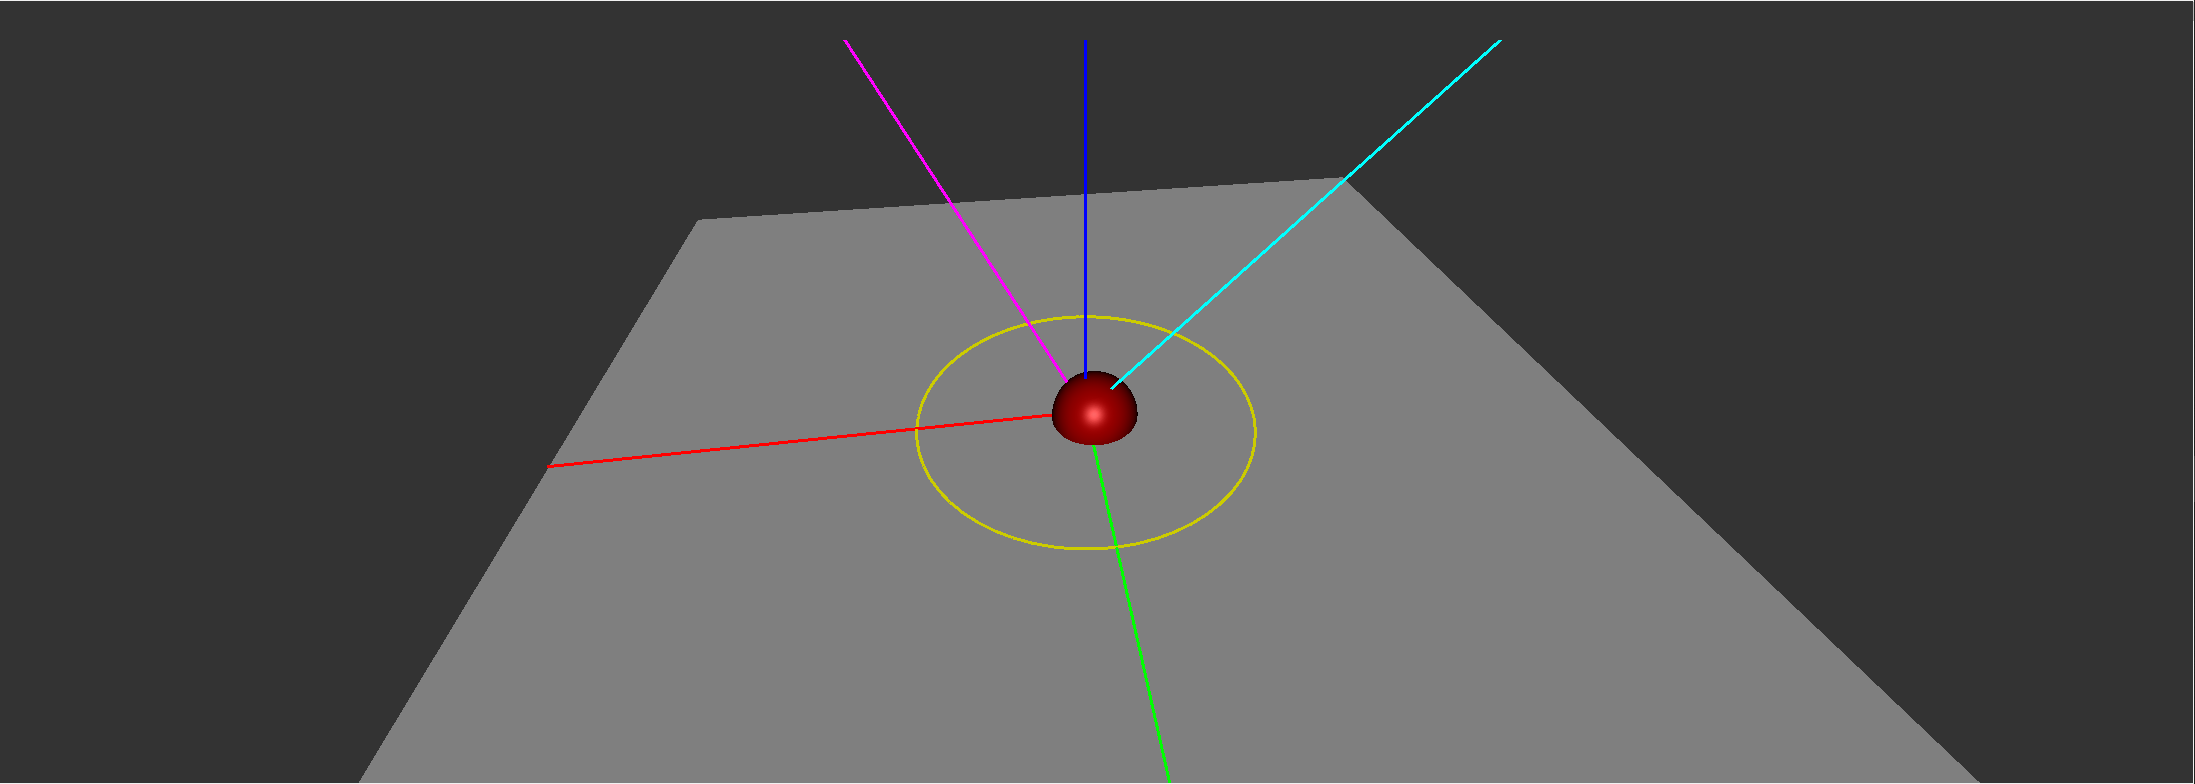
\includegraphics[width=\linewidth]{./Imagens/brdfs/oren-nayar-3D-plot}
    % \vspace{0.1px}
    \legend{ \small (a) 3D \textit{plot}}
\endminipage\hfill
\minipage{0.48\textwidth}
  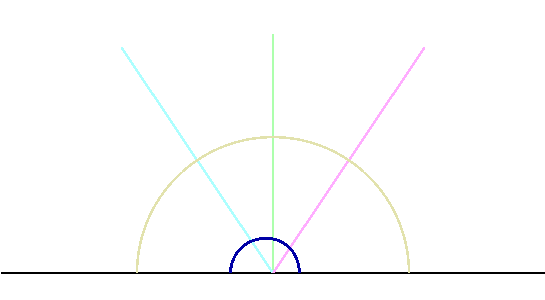
\includegraphics[width=\linewidth]{./Imagens/brdfs/oren-nayar-polar-plot.png}
    \legend{ \small (b) \textit{Polar plot}}
\endminipage\hfill
\end{figure}

\begin{figure}[H]
    \caption{\small{Objetos 3D renderizados pelo experimento Oren-Nayar.}}
    \label{fig-oren-nayar-eqlang}
\minipage{0.32\textwidth}
  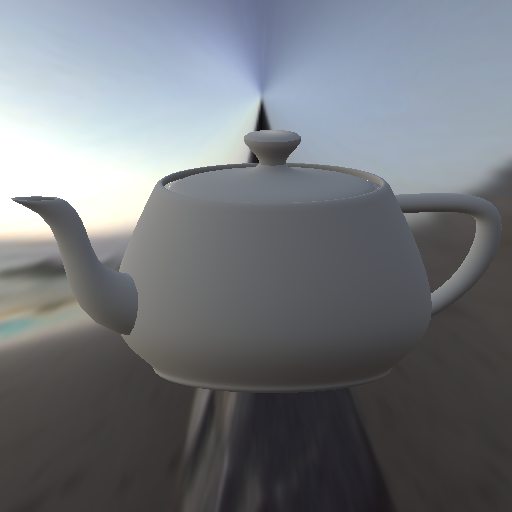
\includegraphics[width=\linewidth]{./Imagens/brdfs/oren-nayar-teapot.png}
    \legend{ \small (a) \textit{Teapot}}
\endminipage\hfill
\minipage{0.32\textwidth}
  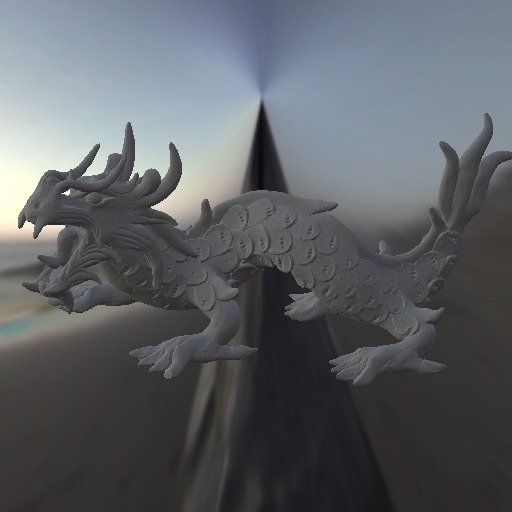
\includegraphics[width=\linewidth]{./Imagens/brdfs/oren-nayar-dragon.png}
    \legend{ \small (b) Dragão de Stanford}
\endminipage\hfill
\minipage{0.32\textwidth}%
  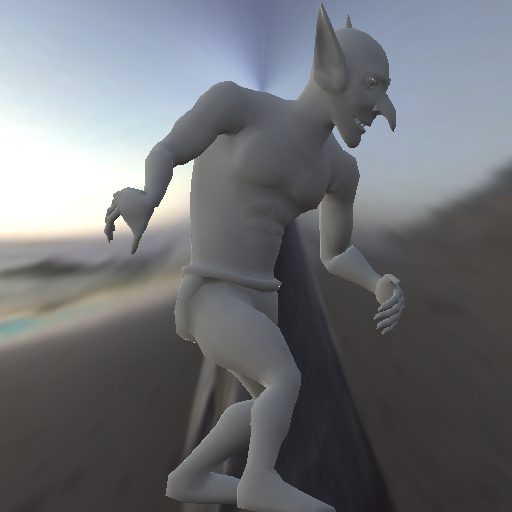
\includegraphics[width=\linewidth]{./Imagens/brdfs/oren-nayar-goblin.png}
    \legend{ \small (c) Goblin}
\endminipage
\end{figure}

